\begin{figure}[b!]
    \centering
    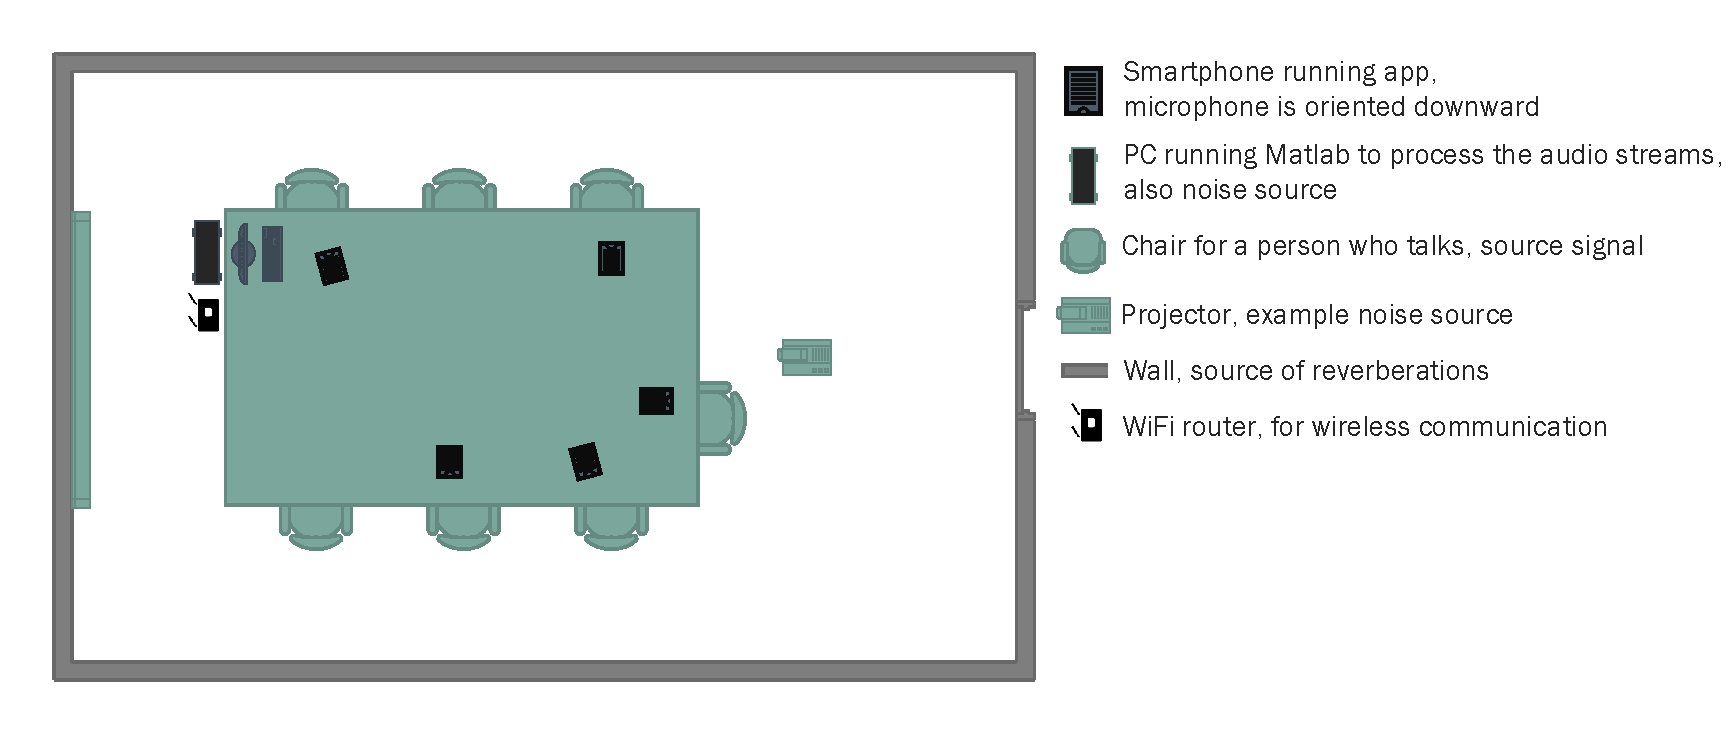
\includegraphics[width=15cm]{images/usage_scenario.pdf}
    \caption{An example usage scenario of the system}
    \label{fig:SchemUsage}
\end{figure}

Voice conferencing with high audio quality has historically required controlled acoustic environments and expensive specialized hardware. However, given the proliferation of smartphones with high-speed networking, fast processors and a variety of sensors, audio quality for a voice conference could now also be improved through combining the audio signals from the participants' smartphones.

Combining audio signals to reject interfering signals is known as \textit{beamforming}. Recent studies have attempted to leverage the availability of smartphones in order to perform (blind) acoustic beamforming \cite{Gaubitch2014, pertila2013} using the integrated microphones. However, Pertila et al.\ do not take into account microphone directivity in their beamforming algorithm and only present results for a delay-and-sum beamformer (DSB) \cite{pertila2013}. Gaubitch et al.\ compensate for these microphone directivities in a minimum variance distortionless response (MVDR) beamformer and demonstrate improved quality \cite{Gaubitch2014} but lack comparison to other widespread beamforming algorithms such as DSB, filter-and-sum \cite[p.~9]{naylor2010speech} or a novel ``Delft beamformer'' \cite{martinez2015}.

Our work will focus on implementing several beamforming algorithms, namely DSB, MVDR and the ``Delft'' beamformers. An example system configuration is shown in figure \ref{fig:SchemUsage}. A number of smartphones are placed on a table in arbitrary but known positions, as well as arbitrary unknown orientations. A number of desired sources (speakers in the conference call) are present, as are several undesired sources (background noise or speakers not part of the conference). The positions of these desired and undesired sources is assumed to be known. The smartphones relay their microphone data, as well as other pertinent information such as timestamps and estimated orientation, to a central computer running \matlab. This computer processes the audio, producing a single enhanced output stream that can be used for voice conferencing, as well as other applications such as automated voice recognition for transcribing a meeting.

The rest of this literature review is structured as follows. In section \ref{sec:android}, several technological barriers to overcome on the smartphone will be presented: application development, clock synchronization, processing latency and orientation estimation. Section \ref{sec:microphone} will focus on the measurement of smartphone microphone directivities and algorithms for interpolation of these measurements. In section \ref{sec:beamforming} the various beamforming algorithms discussed above will be outlined with the intent of running them on a central computer.